\chapter{Data Validation Testing}

	The most common web application security weakness is the failure to properly validate input coming 
	from the client or environment before using it.  Data validation is the task of testing all the 
	possible forms of input, to understand if the application sufficiently validates input data before 
	using it.

\section{Cross Site Scripting (XSS)}

	In Cross Site Scripting (XSS) testing, we test if it is possible to manipulate the input parameters 
	of the application so that it generates malicious output. We find an XSS vulnerability when the
	application does not validate our input and creates an output that is under our control. 

	\subsection{Refelcted Cross Site Scripting}
		Reflected XSS attacks are also known as {\bf type 1 or non-persistent XSS} attacks, and are 
		the most frequent type of XSS attacks found nowadays.
		When a web application is vulnerable to this type of attack, it will pass unvalidated input 
		sent through requests to the client. The common modus operandi of the attack includes a design 
		step, in which the attacker creates and tests an offending URI, a social engineering step, 
		in which she convinces her victims to load this URI on their browsers, and the eventual execution 
		of the offending code — using the victim's credentials.

		One of the important matters about exploiting XSS vulnerabilities is {\bf character encoding}. 
		In some cases, the web server or the web application could not be filtering some encodings of
		characters, so, for example, the web application might filter out a script tag, but might not 
		filter \%3cscript\%3e which simply includes another encoding of tags. 

		{\bf Example:}

		consider a site that has a welcome notice " Welcome \%username\% " and a download link.


		\begin{figure}[H]
			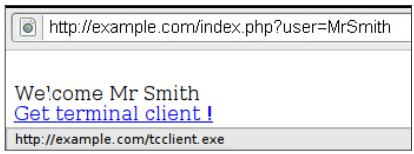
\includegraphics[scale=0.5]{pics/xxs1.png}
		\end{figure}

		To analyze it, the tester will play with the user variable and try to trigger the vulnerability. 
		Let's try to click on the following link and see what happens: 

		\begin{figure}[H]
			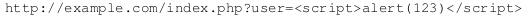
\includegraphics[scale=0.5]{pics/link.png}
		\end{figure}
		If no sanitization is applied this will result in the following popup:

		\begin{figure}[H]
			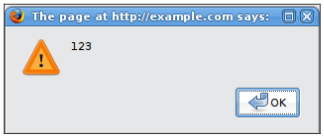
\includegraphics[scale=0.5]{pics/xss2.png}
		\end{figure}

		This indicates that there is an XSS vulnerability and it appears that the tester can execute 
		code of his choice in anybody's browser if he clicks on the tester's link.

	\clearpage
	\subsection{Stored Cross Site Scripting}

		Stored Cross Site Scripting (XSS) is the most dangerous type of Cross Site Scripting. 
		Web applications that allow users to store data are potentially exposed to this type of 
		attack. Stored XSS occurs when a web application gathers input from a user which might 
		be malicious, and then stores that input in a data store for later use. The input that 
		is stored is not correctly filtered. As a consequence, the malicious data will appear
		to be part of the web site and run within the user’s browser under the privileges of the 
		web application. Stored XSS does not need a malicious link to be exploited. 
		A successful exploitation occurs when a user visits a page with a stored XSS.

		The first step is to identify all points where user input is stored into the back-end and 
		then displayed by the application. Typical examples of stored user input can be found in:
		User/Profiles page, shopping cart, file managers, application settings/preferences, etc.

		{\bf Example: }

		\begin{figure}[H]
			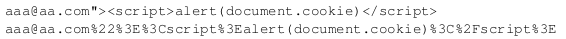
\includegraphics[scale=0.5]{pics/link2.png}
		\end{figure}
		\begin{figure}[H]
			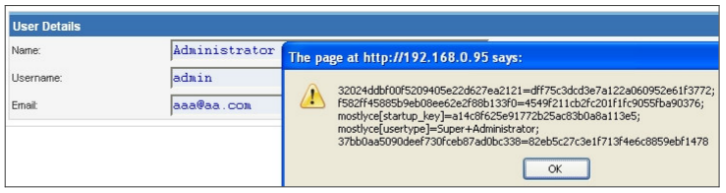
\includegraphics[scale=0.5]{pics/xss3.png}
		\end{figure}


	\subsection{DOM based Cross Site Scripting}
		Not all XSS bugs require the attacker to control the content returned from the server, but 
		can rather abuse poor JavaScript coding practices to achieve the same results. 
		The results are the same as a typical XSS bug, only the means of delivery is different.
		In comparison to other cross site scripting vulnerabilities (reflected and stored XSS), 
		where an unsanitized parameter is passed by the server, returned to the user and executed 
		in the context of the user’s browser, a DOM based cross site scripting vulnerability controls 
		the flow of the code by using elements of the Document Object Model (DOM) along with code 
		crafted by the attacker to change the flow.

		An attacker may append \# \textless script\textgreater alert('xss')\textless /script\textgreater to the affected page URL which would, 
		when executed display the alert box. In this instance, the appended code would not be sent 
		to the server as everything after the \# character is not treated as part of the query by 
		the browser but yet as a fragment. In this example the code is immediately executed and an
		alert of "xss" is displayed in the page. Unlike the more common types of cross site scripting 
		(persistent and non-persistent), in which the code is sent to the server and redisplayed to 
		the user, this is immediately executed in the user’s browser.


	\subsection{Cross Site Flashing}
	**RELEVANT?**

\section{SQL Injections (SQLi)}
	


\section{Buffer Overflow}

	\subsection{Heap Overflow}

	\subsection{Stack Overflow}

	\subsection{Format String}

\section{Other}

	\subsection{Code Injection}

	\subsection{XML Injection}

